\documentclass[../DraftNotes.tex]{subfiles}

\begin{document}

The in class work mainly focused on the deployment of functions. As said, the main functionality provided by FogFaas is the secure deployment of functions on an infrastructure: to get this, we provide a \emph{placeApp} predicate. As an app is a list of services, the predicate call internally the \emph{placeService} predicate, which in turn calls the \emph{placeFunctions} one. Here (parallel or sequential) functions are deployed, according to the resources and the security guarantees of the nodes.
The codebase also embed the trust model of SecFog and can be customized with different trust models. Except for this, basic functionalities of FogFaas don't require a probabilistic reasoning (while, as we'll see in the following, probability plays a key role in modelling communication). \\
In this preliminary work, we had a quite simple type system and few language constructs. The language has been later extended with several instructions, as well as for the type system which provides some new rules.

\subsection{Example: testing FogFaas basic functionalities}
As a main example, we provide a set of services and a complete lattice (in particular a strict total order) as a labelling, as shown in fig.~\ref{fig:tot_order}.

\begin{figure}
	\begin{center}
	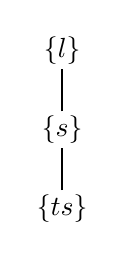
\begin{tikzpicture}
    	\node (top) at (0,0) {$\{ts\}$};
    	\node (med) at (0,1) {$\{s\}$};
    	\node (bot) at (0,2) {$\{l\}$};
    	\draw [thick, shorten <=-2pt, shorten >=-2pt] (top) -- (med);
    	\draw [thick, shorten <=-2pt, shorten >=-2pt] (med) -- (bot); 
	\end{tikzpicture}
	\caption{Default lattice}
  	\label{fig:tot_order}
  	\end{center}
\end{figure}

This can be easily defined by the user by providing a suitable definition of the \emph{labelF} predicate as follows:

\begin{verbatim}
	labelF(default, Args, ts).
	labelF(default, Args, s) :- 
                    findall(X, ts(X, Args), []).
	labelF(default, Args, l) :- 
                    findall(X, notPublic(X, Args), []).
\end{verbatim}

As we'll see, more complicated structures can be provided in a similar way: more on this later on. \\
In this case, we just state that
\begin{itemize}
	\item any function can be top secret (in some sense, low level information can always be promoted to a higher level),
	\item a function can be secret iff it does not have top secret arguments,
	\item a function can be low iff it does not have top secret or secret arguments.
\end{itemize}

In order to perform some security checks, in particular for communication between services and access to resources, a \emph{leq} predicate is also required, which mirrors the order relation induced by \emph{labelF}. The main example lattice and the resulting \emph{leq} predicate are provided as default.
\smallskip
As a preliminary example, consider two services and three nodes, defined as follows:

\begin{verbatim}
	service(service1, triggerX, seq(mult, sum), 1, [ubuntu], [eu]).
	service(service2, triggerY, div, 1, [sql], [eu]).
\end{verbatim}

where mult is a low function, sum is a secret function and div is a top secret function.
Here we require that the hosting node is located in Europe and provides Ubuntu for service1 and SQL for service2. Furthermore, we have an indicator of required capabilites, quantified as 1. \\
The infrastructure is as follows:

\begin{verbatim}
	node(n1, amazon, 3, [ubuntu, sql], 
	[python, rust, java, javascript], 0.001, eu).
	encrypted_storage(n1).
	firewall(n1).

	node(n2, amazon, 2, [ubuntu, sql], 
	[python, rust, java, javascript], 0.001, eu).
	encrypted_storage(n2).
	firewall(n2).

	node(n3, amazon, 1, [ubuntu, sql], 
	[python, rust, java, javascript], 0.001, us).
	encrypted_storage(n3).
\end{verbatim}

where 3, 2 and 1 are a representation of the capabilities offered by the nodes. The labelling of nodes is defined through a \emph{labelN} predicate: 

\begin{verbatim}
	labelN(default, N, OpN, Geo, ts) :- 
                            member(Geo, [eu,ch]), 
                            firewall(N), 
                            member(OpN, [amazon, azure]).
	labelN(default, N, OpN, Geo, s) :- 
                            member(Geo, [eu,ch,us]).
	labelN(default, N, OpN, Geo, l) :- 
                            member(Geo, [eu,ch,us,vat]).

\end{verbatim}

By running the query

\begin{verbatim}
query(placeApp(default, app1, SP, FP)).
\end{verbatim}

we get a suitable deployment. Indeed, as shown in fig.~\ref{fig:Prel_deployment} no service is placed on n3, as both the services are required to be deployed in Europe, while nodes n1 and n2 are eligible to host them as the met the top secret security requirements. However, the function \emph{mult} can be deployed on the node n3, as its security level is low and functions has no particular geographical requirements.

\begin{figure}
	\begin{center}
	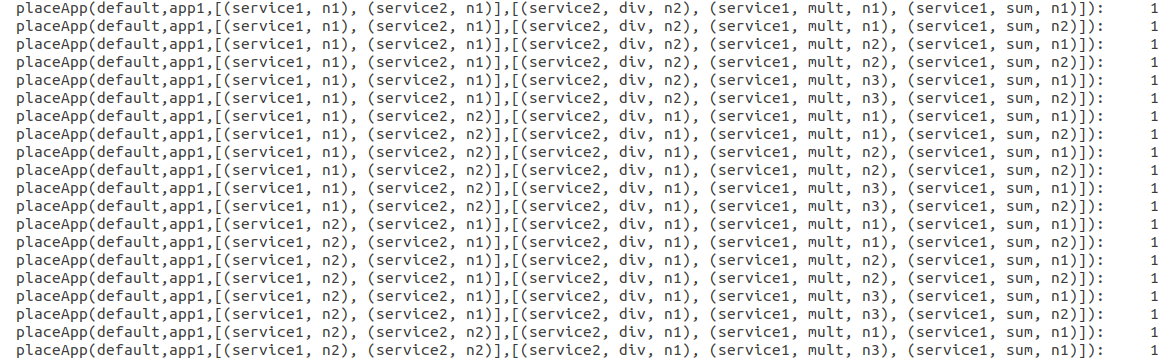
\includegraphics[scale=0.3]{sections/sect_images/Prel_results.png}
	\caption{Possible deployments for the example application}
  	\label{fig:Prel_deployment}
  	\end{center}
\end{figure}

\begin{figure}
	\begin{center}
	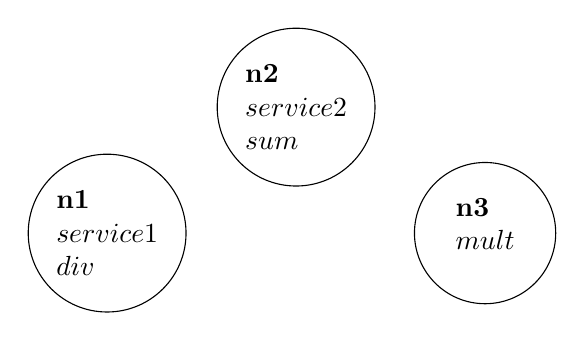
\begin{tikzpicture}
  			[scale=.8,every node/.style={circle}]
  			\node (n1)[draw, align=left] at (3,8)  {\textbf{n1} \\
  									$service1$ \\
  									$div$};
  			\node (n2)[draw, align=left] at (6,10)  {\textbf{n2} \\
  									$service2$ \\
  									$sum$};
  			\node (n3)[draw, align=left] at (9,8) {\\ \textbf{n3} \\
  									$mult$ \\};
	\end{tikzpicture}
	\caption{Graphical representation of a possible deployment}
  	\label{fig:Graph_deployment}
  	\end{center}
\end{figure}

\end{document}